\documentclass[a4paper,14pt,russian]{article}
\usepackage{../MyPackages/commands}
\usepackage[T2A]{fontenc}
\RequirePackage{caption}
\usepackage{graphicx}
\newcommand{\Pn}[3]{P^{(#1)} \br{#2,#3}}
\newcommand{\G}{\Gamma}
\newcommand{\e}{\eta_i^{(1)}}
\newcommand{\ee}{\eta_i^{(2)}}
\renewcommand{\b}{b^{(1)}}
\newcommand{\bb}{b^{(2)}}
\renewcommand{\P}[2]{P\br{\left. #1 \right| #2}}
\newcommand{\iakt}{[\tau_{i},\tau_{i+1})}
\newcommand{\Gr}[1]{\Gamma^{(#1)}}
\newcommand{\Mark}[0]{\brrr{\br{\G_i, \vk_{1,i}, \vk_{2,i}}, \vk_{3,i}, \vk_{4,i}, i \geqslant 0}}
%\newcommand{\Markk}[0]{\brrr{ \vk_i, i \geqslant 0}}
%\newcommand{\Markkhat}[0]{\brrr{ \hat{\vk}_i, i \geqslant 1}}
%\newcommand{\Markkhata}[0]{\brrr{ \hat{\vk}_i\br{a}, i \geqslant 1}}
%\newcommand{\Markkhato}[0]{\brrr{ \hat{\vk}_i\br{0}, i \geqslant 1}}
%\newcommand{\Markkhatoa}[0]{\brrr{ \hat{\hat{\vk}}_i\br{a}, i \geqslant 1}}
\usepackage[Magistr]{../MyPackages/ptvstyle}
\title{Моделирование и анализ системы обслуживания конфликтных потоков в классе приоритетных алгоритмов}
\author{студент группы 85М1\\ Кочеганов В.~М.}
\advisor{к.ф.-м.н., доцент \\ Зорин А.~В.}
\chief{д.ф.-м.н., профессор \\ Федоткин М.~А.}
\date{2013}
\newcommand{\p}{\hat{p}}
\newcommand{\gam}[2]{\Gamma^{\left( #1 , #2 \right)} }
\newcommand{\T}[2]{T^{\left( #1 , #2 \right)} }
\newcommand{\ga}[1]{\Gamma^{\left( #1 \right)} }
\newcommand{\Tt}[1]{T^{\left( #1 \right)} }
\begin{document}

\section{Постановка задачи и построение математической модели}
\subsection{Постановка задачи}

\begin{figure}[h]
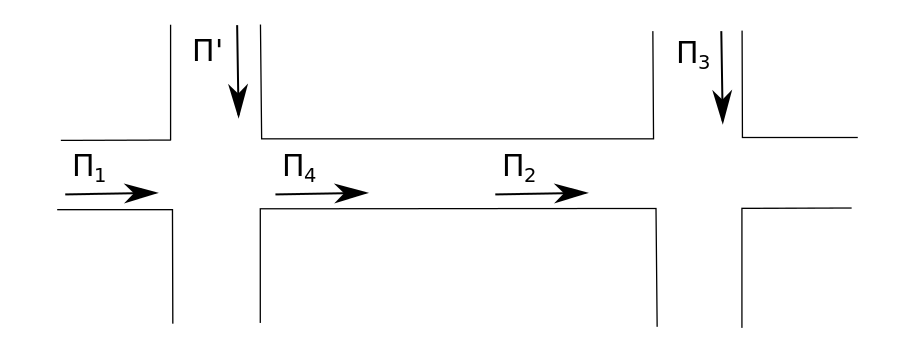
\includegraphics[scale=0.5]{Crossroads.png} 
\end{figure}

\begin{figure}[h]
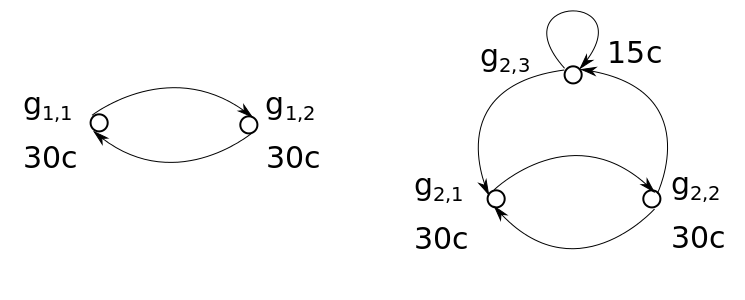
\includegraphics[scale=0.5]{SystemStates.png} 
\end{figure}



Требования по потокам $\Pi_j$, $j=1,2,4$, поступают пачками, причем пачки поступают в соответствии с Пуассоновским процессом с параметром $\la_j$. Требования из потока $\Pi_1$, будучи обслуженными, образуют поток $\Pi_3$.
Требования по потоку $\Pi_j$ поступают в соответствующую очередь $O_j$, $j=\overline{1,4}$.

Первый перекресток может находиться в одном из двух состояний:
\begin{itemize}
\item обслуживать поток $\Pi_1$ (состояние $\gam{1}{1}$ длительностью $\T{1}{1}$) и 
\item
обслуживать поток $\Pi_2$ (состояние $\gam{1}{2}$ длительностью $\T{1}{2}$).
\end{itemize}

Второй перекресток имеет три состояния:
\begin{itemize}
\item обслуживание потока $\Pi_3$ (состояние $\gam{2}{1}$ длительностью $\T{2}{1}$);
\item обслуживание потока $\Pi_4$ (состояние $\gam{2}{2}$ длительностью $\T{2}{2}$) и
\item продолжение обслуживания потока $\Pi_4$ в случае 
превышения объема оставшейся очереди $O_4$ некого порога (состояние $\gam{2}{3}$ длительностью $\T{2}{3}$);
\end{itemize}


Объединим рассматриваемые обслуживающие устройства в одно, состояние которого опишем с помощью вектора из множества $S_{general}\left(\Gamma^{(1,i_1)}; \Gamma^{(2,i_2)}; T\right)$, где $i_1\in \left\{1,2\right\}$, $i_2 \in \left\{1,2,3\right\}$, $T\in \left\{1, 2, \ldots, \max_{i_1,i_2}{\left(T^{(1,i_1)}, T^{(2,i2)}\right)}\right\}$. Свое состояние новое устройство меняет в моменты смены состояний одного из составляющих его устройств.

\begin{theorem}
Количество состояний полученного обслуживающего устройства конечно
\end{theorem}
\begin{proof}
Поскольку множество различных состояний $\Gamma$, в которые обслуживающее устройство может совершить переход, является подмножеством $S_{general}$ ($S \subset S_{general}$), то
\begin{equation*}
\left|S\right| \leqslant \left|S_{general}\right| = 2\times 3 \times \max_{i_1,i_2}{\left(T^{(1,i_1)}, T^{(2,i2)}\right)}
\end{equation*}
\end{proof}

В следствие этого результата мы можем перенумеровать состояния $\G = \brrr{\G^{(1)},\G^{(2)}, \ldots, \G^{(n)}}$, а также соответствующие им длительности $T=\brrr{T^{(1)},T^{(2)}, \ldots, T^{(n)}}$.
Каждое состояние $\G^{(r)}$ принадлежит одному из следующих четырех классов $\G^{\Rmnum{1}}$, $\G^{\Rmnum{2}}$, $\G^{\Rmnum{3}}$ и $\G^{\Rmnum{4}}$.
\begin{itemize}
\item в состоянии $\G^{(r)} \in \G^{\Rmnum{1}}$ обслуживаются только требования из очередей $O_1$ и $O_3$;
\item в состоянии $\G^{(r)} \in \G^{\Rmnum{2}}$ обслуживаются только требования из очередей $O_1$ и $O_4$;
\item в состоянии $\G^{(r)} \in \G^{\Rmnum{3}}$ обслуживаются только требования из очередей $O_2$ и $O_3$;
\item в состоянии $\G^{(r)} \in \G^{\Rmnum{4}}$ обслуживаются только требования из очередей $O_2$ и $O_4$.
\end{itemize}

Для описания процесса обслуживания будут также использоваться потоки насыщения $\Pi^{sat}_j$, $j=\overline{1,4}$, определяемые как выходные потоки при максимальной загруженности обслуживающего устройства. Пусть
\begin{itemize}
\item для $j=1$ $^j\G=\G^{\Rmnum{1}} \bigcup \G^{\Rmnum{2}}$;
\item для $j=2$ $^j\G=\G^{\Rmnum{3}} \bigcup \G^{\Rmnum{4}}$;
\item для $j=3$ $^j\G=\G^{\Rmnum{1}} \bigcup \G^{\Rmnum{3}}$;
\item для $j=4$ $^j\G=\G^{\Rmnum{2}} \bigcup \G^{\Rmnum{4}}$;
\end{itemize}
Тогда поток насыщения $\Pi^{sat}_j$ будет содержать неслучайное число $l_{r,j}$ требований, обслуженных в течение времени $\Tt{r}$, если $\ga{r} \in ^j\G$, и не будет содержать требований в противном случае, $\ga{r} \notin ^j\G$. 

Моменты $\tau_0 = 0, \tau_1, \ldots$ наблюдения за системой положим совпадающими с моментами переключения состояния обслуживающего устройства. Определим следующие случайные величины и элементы:
\begin{itemize}
\item количество $\vk_{j,i} \in Z_+ $ требований в очереди $O_j$ в момент времени $\tau_i$;
\item состояние обслуживающего устройства $\G_i\in \G = \brrr{\G^{(1)},\G^{(2)}, \ldots, \G^{(n)}}$ в течение $\left(\tau_{i-1};\tau_i\right]$;
\item количество $\eta_{j,i}$ требований, поступивших в очередь $O_j$ по потоку $\Pi_j$ в течение $\left(\tau_{i};\tau_{i+1}\right]$;
\item количество $\xi_{j,i}$ требований по потоку насыщения $\Pi^{sat}_j$ в течение $\left(\tau_{i};\tau_{i+1}\right]$;
\item количество $\overline{\xi_{j,i}}$ реально обслуженных требований по потоку $\Pi_j$.
\end{itemize}

\subsection{Свойства условных распределений}
Будем считать, что закон изменения состояния обслуживающего устройства нам известен и задается следующей функцией:
\begin{equation*}
\G_{i+1} = h(\G_i,\vk_{4,i}).
\end{equation*}
Также для определения длительности $T_{i}$ состояния обслуживающего устройства в течение $\left(\tau_{i-1};\tau_i\right]$, удобно ввести следующую функцию:
\begin{equation}
T_{i+1}=h_T(\G_i,\vk_{4,i})= \Tt{r'},\quad  \text{ где } \ga{r'}=h(\G_i,\vk_{4,i}).
\label{timeLaw}
\end{equation}

Тогда имеем
\begin{align}
\overline{\xi}_{j,i} = \min{\brrr{\xi_{j,i},\vk_{j,i}+\eta_{j,i}}}&,\quad \vk_{i+1}=\max{\brrr{0,\vk_{j,i}+\eta_{j,i}-\xi_{j,i}}}\nonumber \\
\G_{i+1}=h(\G_i,\vk_{4,i})&,\quad \eta_{3,i}=\overline{\xi_{1,i}} = \vk_{1,i}+\eta_{1,i} + \min{\brrr{0,\xi_{1,i} - \br{\vk_{1,i}+\eta_{1,i}}}}.
\label{deterministicLaw}
\end{align}

Обозначим через $\vp_j(x,t)$ вероятность того, что за время $t>0$ по потоку $\Pi_j$ поступит ровно $x\in Z_+$ требований:
\begin{equation}
\P{\brrr{\omega\colon \eta_{j,i} = b}}{\brrr{\omega\colon \G_i=\ga{r}, \vk_{4,i}=x}}=\vp_j(b,T_{i+1}).
\end{equation}

Учитывая закон распределения процесса Пуассона и количества требований в пачках, величины $\vp_j(x,t)$ могут быть найдены из соотношений
\begin{equation}
\sum_{x=0}^{\infty} z^x\vp_j(x,t) = exp\brrr{\la_j t \br{\sum_{b=1}^{\infty} z^b \pi(b,j) -1}}
\end{equation}

Для потоков насыщения имеем следующие соотношения:
\begin{align}
\P{\xi_{j,i} = 0}{\G_i=\ga{r}} = 1, &\quad \G_{i+1}\notin ^j\G,\\
\P{\xi_{j,i} = l_{r',j}}{\G_i=\ga{r}} = 1, &\quad \G_{i+1}=\ga{r'}\in ^j\G,
\end{align}
где $j=\overline{1,4}$.

Введем следующие события:
\begin{align}
A_i\br{r;x_1;x_2;x_3;x_4} &= \brrr{\G_i=\ga{r},\vk_{4,i}=x_4}\bigcap \brrr{\vk_{1,i}=x_1,\vk_{2,i}=x_2,\vk_{3,i}=x_3}\\
B_i\br{b_1;b_2;b_4;y_1;y_2;y_3;y_4} &= \brrr{\eta_{1,i}=b_1,\eta_{2,i}=b_2,\eta_{4,i}=b_4,\xi_{1,i}=y_1,\xi_{2,i}=y_2,\xi_{3,i}=y_3,\xi_{4,i}=y_4}
\end{align}

В соответствии с описанной структурой системы, количество требований пришедших по потокам $\Pi_1$, $\Pi_2$, $\Pi_4$, $\Pi_1^{out}$, $\Pi_2^{out}$, $\Pi_3^{out}$ и $\Pi_4^{out}$ за $(i+1)$-ый такт зависит лишь от состояния обслуживающего устройства и размера очередей $O_j$, $j=\overline{1,4}$, в момент $\tau_i$. Поэтому условные распределения рассматриваемых в системе потоков, учитывая все <<прошлое>> системы можно расписать следующим образом:
\ml
{
\label{etaXiIndependence}
\P{B_i\br{b_1;b_2;b_4;y_1;y_2;y_3;y_4}}{\bigcap_{t=0}^{i} A_t\br{r_t;x_{1,t};x_{2,t};x_{3,t};x_{4,t}}} = \\
= \P{\eta_{1,i}=b_1, \eta_{2,i}=b_2, \eta_{4,i}=b_4, \xi_{1,i}=y_1, \xi_{2,i}=y_2, \xi_{3,i}=y_3, \xi_{4,i}=y_4}{\G_i=\ga{r_i},\vk_{4,i}=x_{4,i}}=\\
= \P{\eta_{1,i}=b_1}{\G_i=\ga{r_i},\vk_{4,i}=x_{4,i}} \times
\P{\eta_{2,i}=b_2}{\G_i=\ga{r_i},\vk_{4,i}=x_{4,i}} \times \\
\P{\eta_{4,i}=b_4}{\G_i=\ga{r_i},\vk_{4,i}=x_{4,i}} \times 
\P{\xi_{1,i}=y_1}{\G_i=\ga{r_i},\vk_{4,i}=x_{4,i}} \times \\
\P{\xi_{2,i}=y_2}{\G_i=\ga{r_i},\vk_{4,i}=x_{4,i}} \times
\P{\xi_{3,i}=y_3}{\G_i=\ga{r_i},\vk_{4,i}=x_{4,i}} \times \\
\P{\xi_{4,i}=y_4}{\G_i=\ga{r_i},\vk_{4,i}=x_{4,i}}
}

В завершение построении математической модели рассматриваемой системы сформулируем и докажем следующую теорему:
\begin{theorem}
При заданном распределении начального вектора $\br{\G_0,\vk_{1,0},\vk_{2,0},\vk_{3,0},\vk_{4,0}}$ последовательность $\Mark$ является цепью Маркова. 
\end{theorem}

\begin{proof}
Для доказательства достаточно показать, что 
\ml
{
\P{A_{i+1}\br{r;x_{1};x_{2};x_{3};x_{4}}}{\bigcap_{t=0}^{i} A_t\br{r_t;x_{1,t};x_{2,t};x_{3,t};x_{4,t}}} = \\
\P{A_{i+1}\br{r;x_{1};x_{2};x_{3};x_{4}}}{ A_i\br{r_i;x_{1,i};x_{2,i};x_{3,i};x_{4,i}}}
\label{markovToProve}
}
Распишем сначала левую часть равенства \eqref{markovToProve}. Учитывая то, что сумма непересекающихся событий $B_i\br{b_1;b_2;b_4;y_1;y_2;y_3;y_4}$ есть достоверное событие $\Omega$, $\bigcup_{b,y} B_i\br{b_1;b_2;b_4;y_1;y_2;y_3;y_4}=\Omega$ получим
\ml
{
\P{A_{i+1}\br{r;x_{1};x_{2};x_{3};x_{4}}}{\bigcap_{t=0}^{i} A_t\br{r_t;x_{1,t};x_{2,t};x_{3,t};x_{4,t}}} = \\
=\sum_{b,y}\P{A_{i+1}\br{r;x_{1};x_{2};x_{3};x_{4}} \bigcap B_i\br{b_1;b_2;b_4;y_1;y_2;y_3;y_4}}{\bigcap_{t=0}^{i} A_t\br{r_t;x_{1,t};x_{2,t};x_{3,t};x_{4,t}}} = \\
= \sum_{b,y}\P{B_i\br{b_1;b_2;b_4;y_1;y_2;y_3;y_4}}{\bigcap_{t=0}^{i} A_t\br{r_t;x_{1,t};x_{2,t};x_{3,t};x_{4,t}}}\times\\
\times \P{A_{i+1}\br{r;x_{1};x_{2};x_{3};x_{4}}}{\bigcap_{t=0}^{i} A_t\br{r_t;x_{1,t};x_{2,t};x_{3,t};x_{4,t}}\bigcap B_i\br{b_1;b_2;b_4;y_1;y_2;y_3;y_4}}
\label{markovProof}
}
Беря во внимание \eqref{deterministicLaw}, найдем второй множитель:
\ml
{
\P{A_{i+1}\br{r;x_{1};x_{2};x_{3};x_{4}}}{\bigcap_{t=0}^{i} A_t\br{r_t;x_{1,t};x_{2,t};x_{3,t};x_{4,t}}\bigcap B_i\br{b_1;b_2;b_4;y_1;y_2;y_3;y_4}} = \\
= P\left(\G_{i+1}=\ga{r},\vk_{1,i+1}=x_1,\vk_{2,i+1}=x_2,\vk_{3,i+1}=x_3,\vk_{4,i+1}=x_4\right| \bigcap_{t=0}^{i-1} A_t\br{r_t;x_{1,t};x_{2,t};x_{3,t};x_{4,t}} \bigcap \\ \bigcap 
\brrr{\G_i=\ga{r_i},\vk_{1,i}=x_{1,i},\vk_{2,i}=x_{2,i},\vk_{3,i}=x_{3,i},\vk_{4,i}=x_{4,i}} \bigcap \\
\bigcap \left. \brrr{\eta_{1,i}=b_1,\eta_{2,i}=b_2,\eta_{4,i}=b_4,\xi_{1,i}=y_1,\xi_{2,i}=y_2,\xi_{3,i}=y_3,\xi_{4,i}=y_4}
\right) = \\
= P\left(h\br{\ga{r_i},x_{4,i}}=\ga{r},
\max{\brrr{0,x_{1,i}+b_1-y_1}}=x_1,
\max{\brrr{0,x_{2,i}+b_2-y_2}}=x_2,\right. \\
\left.
\max{\brrr{0,x_{3,i}+x_{1,i}+b_1 + \min{\brrr{0,x_{1,i} - \br{x_{1,i}+b_1}}} - y_3}}=x_3,
\max{\brrr{0,x_{4,i}+b_4-y_4}}=x_4,\right|\\ 
\bigcap_{t=0}^{i-1} A_t\br{r_t;x_{1,t};x_{2,t};x_{3,t};x_{4,t}} \bigcap 
\brrr{\G_i=\ga{r_i},\vk_{1,i}=x_{1,i},\vk_{2,i}=x_{2,i},\vk_{3,i}=x_{3,i},\vk_{4,i}=x_{4,i}} \bigcap \\
\bigcap \left. \brrr{\eta_{1,i}=b_1,\eta_{2,i}=b_2,\eta_{4,i}=b_4,\xi_{1,i}=y_1,\xi_{2,i}=y_2,\xi_{3,i}=y_3,\xi_{4,i}=y_4}
\right) = \\
= P\left(h\br{\ga{r_i},x_{4,i}}=\ga{r},
\max{\brrr{0,x_{1,i}+b_1-y_1}}=x_1,
\max{\brrr{0,x_{2,i}+b_2-y_2}}=x_2,\right. \\
\left.
\max{\brrr{0,x_{3,i}+x_{1,i}+b_1 + \min{\brrr{0,x_{1,i} - \br{x_{1,i}+b_1}}} - y_3}}=x_3,
\max{\brrr{0,x_{4,i}+b_4-y_4}}=x_4,\right),
\label{markovProoff}
}
где последнее равенство верно, поскольку оставшаяся под знаком вероятности величина уже не является случайной. Из \eqref{etaXiIndependence}, \eqref{markovProof} и  \eqref{markovProoff} получаем выражение для левой части равенства \eqref{markovToProve}:
\ml
{
\P{A_{i+1}\br{r;x_{1};x_{2};x_{3};x_{4}}}{\bigcap_{t=0}^{i} A_t\br{r_t;x_{1,t};x_{2,t};x_{3,t};x_{4,t}}} = \\
=  \sum_{b,y}\P{\eta_{1,i}=b_1, \eta_{2,i}=b_2, \eta_{4,i}=b_4, \xi_{1,i}=y_1, \xi_{2,i}=y_2, \xi_{3,i}=y_3, \xi_{4,i}=y_4}{\G_i=\ga{r_i},\vk_{4,i}=x_{4,i}}\times\\
\times  P\left(h\br{\ga{r_i},x_{4,i}}=\ga{r},
\max{\brrr{0,x_{1,i}+b_1-y_1}}=x_1,
\max{\brrr{0,x_{2,i}+b_2-y_2}}=x_2,\right. \\
\left.
\max{\brrr{0,x_{3,i}+x_{1,i}+b_1 + \min{\brrr{0,x_{1,i} - \br{x_{1,i}+b_1}}} - y_3}}=x_3,
\max{\brrr{0,x_{4,i}+b_4-y_4}}=x_4,\right)
}

Заметим, что в наших рассуждениях мы нигде не использовали информацию о событиях \par $\bigcap_{t=0}^{i-1} A_t\br{r_t;x_{1,t};x_{2,t};x_{3,t};x_{4,t}}$, поэтому рассуждения для правой части \eqref{markovToProve} будут аналогичными:
\mll
{
\P{A_{i+1}\br{r;x_{1};x_{2};x_{3};x_{4}}}{ A_i\br{r_i;x_{1,i};x_{2,i};x_{3,i};x_{4,i}}} = \\
= \sum_{b,y}\P{B_i\br{b_1;b_2;b_4;y_1;y_2;y_3;y_4}}{ A_i\br{r_i;x_{1,i};x_{2,i};x_{3,i};x_{4,i}}}\times\\
\times \P{A_{i+1}\br{r;x_{1};x_{2};x_{3};x_{4}}}{ A_i\br{r_i;x_{1,i};x_{2,i};x_{3,i};x_{4,i}}\bigcap B_i\br{b_1;b_2;b_4;y_1;y_2;y_3;y_4}} = \\
= \sum_{b,y}\P{\eta_{1,i}=b_1, \eta_{2,i}=b_2, \eta_{4,i}=b_4, \xi_{1,i}=y_1, \xi_{2,i}=y_2, \xi_{3,i}=y_3, \xi_{4,i}=y_4}{\G_i=\ga{r_i},\vk_{4,i}=x_{4,i}}\times \\
\times 
P\left(\G_{i+1}=\ga{r},\vk_{1,i+1}=x_1,\vk_{2,i+1}=x_2,\vk_{3,i+1}=x_3,\vk_{4,i+1}=x_4\right|  \\ 
\brrr{\G_i=\ga{r_i},\vk_{1,i}=x_{1,i},\vk_{2,i}=x_{2,i},\vk_{3,i}=x_{3,i},\vk_{4,i}=x_{4,i}} \bigcap \\
\bigcap \left. \brrr{\eta_{1,i}=b_1,\eta_{2,i}=b_2,\eta_{4,i}=b_4,\xi_{1,i}=y_1,\xi_{2,i}=y_2,\xi_{3,i}=y_3,\xi_{4,i}=y_4}
\right) = 
}
откуда опять в силу \eqref{deterministicLaw} получаем
\mll
{
=\sum_{b,y}\P{\eta_{1,i}=b_1, \eta_{2,i}=b_2, \eta_{4,i}=b_4, \xi_{1,i}=y_1, \xi_{2,i}=y_2, \xi_{3,i}=y_3, \xi_{4,i}=y_4}{\G_i=\ga{r_i},\vk_{4,i}=x_{4,i}}\times \\
\times P\left(h\br{\ga{r_i},x_{4,i}}=\ga{r},
\max{\brrr{0,x_{1,i}+b_1-y_1}}=x_1,
\max{\brrr{0,x_{2,i}+b_2-y_2}}=x_2,\right. \\
\left.
\max{\brrr{0,x_{3,i}+x_{1,i}+b_1 + \min{\brrr{0,x_{1,i} - \br{x_{1,i}+b_1}}} - y_3}}=x_3,
\max{\brrr{0,x_{4,i}+b_4-y_4}}=x_4,\right).
}
Таким образом, выражения для левой и правой частей \eqref{markovToProve} совпадают, следовательно равенство верно и последовательность $\Mark$ является цепью Маркова.
\end{proof}
\end{document}
